\documentclass[11pt, oneside]{article}   	% use "amsart" instead of "article" for AMSLaTeX format
\usepackage{geometry}                		% See geometry.pdf to learn the layout options. There are lots.
\geometry{letterpaper}                   		% ... or a4paper or a5paper or ...
%\geometry{landscape}                		% Activate for rotated page geometry
%\usepackage[parfill]{parskip}    		% Activate to begin paragraphs with an empty line rather than an indent
\usepackage{graphicx}
\usepackage{amssymb}
\usepackage[francais]{babel}
\usepackage[utf8]{inputenc} % utile pour les accents !!!


\title{\huge{\textbf{Système Distribué}}}
\author{Blazevic Mehmed \& Orphée Antoniadis}
%\date{}							% Activate to display a given date or no date

\begin{document}
\maketitle
\section{Introduction}
Dans le cadre du cours de système distribué, on nous demande de réaliser un système permettant
de collecter des données d'un réseau de capteurs, afin de pouvoir piloter différent périphériques
fonctionnant avec la technologie Z-Wave.

\newpage
\section{Base de donnée}
Notre modèle de base de donnée est simple et relationnel. Voici un diagramme:

\begin{figure}[!h]
\begin{center}
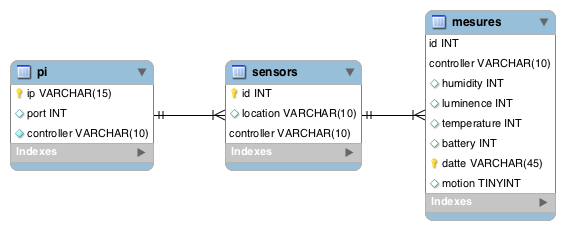
\includegraphics[scale=0.8]{images/distributed_bdd.png}
\end{center}
\end{figure}

\begin{itemize}
    \item \textbf{pi}   :  Pour la table pi, on utilise comme clé une IP sous forme de chaînes
    de caractères. Elle est liée à la table sensors via "controller".
    \item \textbf{sensors} : Cette table utilise id et controller pour former sa clé. Ce dernier
    permettant de la lier à la table pi.
    \item \textbf{mesures} : Contient toutes les mesures effectuées. Chaque mesure pour chaque
    capteur est unique, c'est pour cela que l'on utilise comme clé l'id, le controller \textbf{ET}
    une date "datte". Les attributs id et controller nous permettent de faire le lien avec la table sensors.

\end{itemize}





\end{document}
